\bookchapter{الفصل 37: ثورة النموذج — من «كتابة الكود» إلى «قيادة الذكاء الاصطناعي لكتابة الكود»}

\chapterintro{تهانينا، أنت الآن في قلب ثورة مهنية كبرى. بدأت هذه الثورة بجملة نشرها مبرمج على وسائل التواصل الاجتماعي في 2025. يبدو الأمر دراميًا؟ لكن هذا هو الواقع.}

\booksection{أولاً: ولادة Vibe Coding: حركة بدأت بجملة واحدة}

في فبراير 2025، نشر Andrej Karpathy — احفظ هذا الاسم، ستراه عدة مرات — تغريدة على وسائل التواصل الاجتماعي لاقت اقتباسات كثيرة: «هناك طريقة برمجة جديدة تسمى Vibe Coding، تعتمد تمامًا على الإحساس (vibes)، وتتجاهل تفاصيل الكود، وتدعِ الذكاء الاصطناعي يتولى كل شيء. تقول ما تراه، وتنسخ وتلصق، وما دام يعمل فهذا يكفي.»

هذه الملاحظة العابرة سمّت بدقة تحولًا في النموذج كان يحدث بالفعل: لم يعد الإنسان يكتب الكود سطرًا بسطر، بل يصف النية باللغة الطبيعية، ويقوم الذكاء الاصطناعي بالتنفيذ. عبارات Karpathy فيها شيء من السخرية، لكن خلفها رؤية عميقة: عندما تتجاوز قدرة الذكاء الاصطناعي على توليد الكود عتبة معينة، يصبح التحدي ليس «هل أستطيع كتابة هذا السطر؟» بل «هل أستطيع توضيح ما أريده فعلًا؟».

\begin{tcbinfo}{نصيحة: ما معنى Vibe؟}
Vibe تعني حرفيًا «الأجواء، الإحساس». Vibe Coding تعني «قيادة الذكاء الاصطناعي للبرمجة بالإحساس» — تصف ما تريد، والذكاء الاصطناعي يتولى التنفيذ. احفظ هذه الكلمة، فهي «شهادة ميلاد» هذه الثورة.

\end{tcbinfo}

منذ تلك اللحظة، بدأ مفهوم «الترميز» يتشقق: الترميز التقليدي هو ترجمة التصميم إلى صياغة برمجية؛ والترميز الجديد هو ترجمة النية إلى أوامر. الأول يختبر الأصابع، والثاني يختبر العقل.

سرعان ما تحولت Vibe Coding من سخرية إلى مفهوم هندسي جاد. بحلول منتصف 2026، تطورت من نكتة على وسائل التواصل إلى منهجية متكاملة — تغطي التعبير عن المتطلبات وإدارة السياق والتكرار والتحقق وضمان الجودة. وبدأ الناس يدركون أن «الإحساس» مجرد مرحلة تمهيدية، والبرمجة الفعالة بالذكاء الاصطناعي تحتاج إلى تفكير منهجي. وهذه هي المنهجية التي يقدمها لك هذا الكتاب.

\booksection{ثانيًا: واقع 2026: عصر Agentic Engineering}

بحلول أغسطس 2026، مر مجال برمجة الذكاء الاصطناعي بعدة تطورات في النموذج. كانت Vibe Coding الشرارة الأولى، لكن سرعان ما اكتشف الجميع أن «الإحساس» وحده في الدردشة مع الذكاء الاصطناعي يعطي جودة غير مستقرة — أحيانًا مذهلة وأحيانًا فاشلة. فبدأ التطور: من البرمجة الحوارية البسيطة إلى هندسة الوكلاء المنظمة.

ومن جديد Karpathy، طرح في مطلع 2026 مفهوم Agentic Engineering. بخلاف Vibe Coding التي «تقول وتولّد»، تشدد Agentic Engineering على: امنح الذكاء الاصطناعي هدفًا، ودعه يخطط الخطوات ويوظف الأدوات ويوافق النتائج ويعيد التصحيح. لم يعد الذكاء الاصطناعي مجرد مولد كود، بل وكيل ذكي يدرك البيئة ويتخذ القرارات وينفذ الإجراءات.

أدى هذا التحول إلى ثلاثة تغييرات جوهرية:

\begin{enumerate}
  \item تغير نمط التفاعل: من «سؤال وجواب» إلى «تحديد الهدف ثم منح الصلاحية».
  \item تغير المخرجات: من «جزء من الكود» إلى «مشروع كامل».
  \item تغير دور الإنسان: من «مراجعة الكود سطرًا بسطر» إلى «تحديد الحدود والتحقق من النتائج».
\end{enumerate}

الأرقام لا تكذب: في إصدار Cursor 3 الصادر في أبريل 2026، تجاوزت نسبة استخدام وضع Agent وضع إكمال Tab لأول مرة، مما يدل على تحوّل المطورين على نطاق واسع إلى أسلوب العمل هذا؛ أما أداة Claude Code البرمجية الأصلية في الطرف، فقد بلغت إيراداتها السنوية 2.5 مليار دولار بحلول منتصف 2026. يوضح الرسم البياني التالي لحظة التقاطع:

\begin{center}
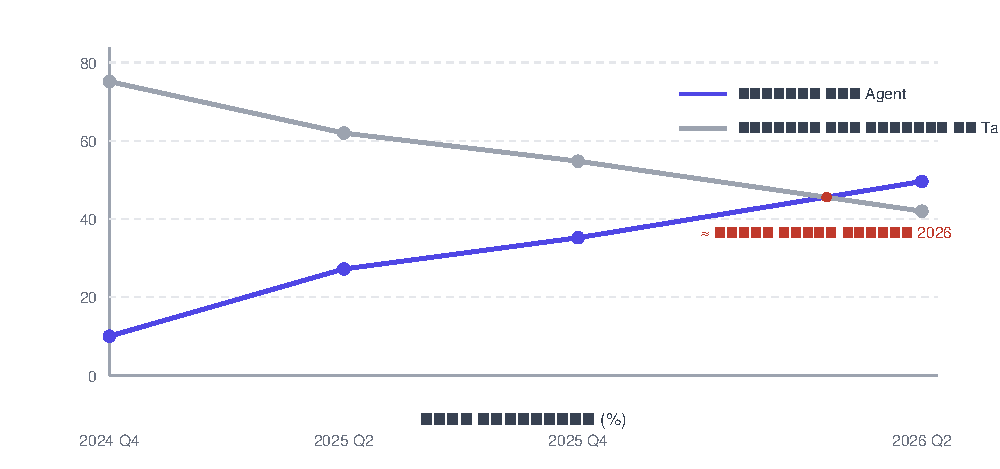
\includegraphics[width=0.92\linewidth]{figures/fig-di-san-shi-qi-zhang-1}
\\[2pt]\small الشكل 1: تغير نسبة استخدام أنماط تفاعل برمجة الذكاء الاصطناعي (تقديرات مبنية على أبحاث الصناعة، الربع الثاني 2026 تجاوز Agent وضع Tab)
\end{center}

لكن بصراحة: تغير الأدوات والنماذج مجرد ظاهر. سواء استخدمت Cursor أو Claude Code، وسواء كان النموذج GPT-5 أم Claude 4.5، فالممارسون الناجحون يتبعون المنهجية نفسها. وهذا ما يعلمه لك هذا الدليل.

\booksection{ثالثًا: التحول المعرفي الجوهري: من Coder إلى Conductor}

تعليم البرمجة التقليدي يعلّمك كيف تكون Coder — تفهم الصياغة وتتذكر واجهات البرمجة وتصحح الأخطاء المنطقية. في عصر برمجة الذكاء الاصطناعي، يُعاد تعريف هذا الدور. لم تعد بحاجة إلى كتابة كل سطر بنفسك، بل تحتاج إلى أن تكون «قائدًا» (Conductor): يحدد ساحة المعركة ويضع القواعد ويوزع المهام ويتحقق من النتائج.

جوهر هذا التحول ليس «هل تعرف كتابة الكود؟» بل «هل تعرف ماذا تريد فعله؟». القائد الجيد ليس بالضرورة أفضل جندي، لكنه الأوضح بشأن هدف المعركة والتضاريس وتوزيع القوى. وبالمثل، الممارس الجيد لبرمجة الذكاء الاصطناعي ليس بالضرورة ملمًا بتفاصيل كل لغة برمجة، لكنه الأوضح بشأن أهداف المشروع وقيوده ومعايير الجودة.

هذا الجدول يستحق القراءة مرتين — إنه يلخص جوهر التحول في الأدوار:

\begin{center}
\begin{tabularx}{\linewidth}{|X|X|X|}
\hline
\textbf{البُعد} & \textbf{Coder التقليدي} & \textbf{قائد الذكاء الاصطناعي (Conductor)} \tabularnewline
\hline
المهارات الأساسية & حفظ الصياغة، واستدعاء واجهات البرمجة، والتصحيح & تحديد المتطلبات، وإدارة السياق، والحكم على النتائج \tabularnewline
أسلوب العمل & كتابة الكود سطرًا بسطر & وصف النية، ومراجعة المخرجات \tabularnewline
ضبط الجودة & ما كتبته بنفسك تعرفه جيدًا & التحقق من مخرجات الذكاء الاصطناعي عبر الاختبارات والمراجعة \tabularnewline
متطلبات المعرفة & إتقان عميق لغة/إطار عمل محدد & فهم واسع للتقنية، وفهم عميق لمنطق العمل \tabularnewline
موقع الاختناق & سرعة الترميز وحفظ الصياغة & وضوح التفكير وقدرة التعبير \tabularnewline
مصدر الخطأ & أخطاء صياغة، إغفالات منطقية & غموض المتطلبات، نقص السياق \tabularnewline
\hline
\end{tabularx}
\end{center}

\begin{center}\small\color{gray}مقارنة أبعاد القدرات بين Coder التقليدي وقائد الذكاء الاصطناعي\end{center}

هذا لا يعني أن معرفة البرمجة أصبحت غير مهمة. بل العكس: عندما تفهم الكود الذي يكتبه الذكاء الاصطناعي، تستطيع مراجعته وتصحيحه بفعالية؛ وعندما تفهم هياكل البيانات والخوارزميات، تستطيع الحكم على مدى معقولية الحل. المعرفة تحدد «سقف قيادتك» — لكن دورها تغير من «أداة تنفيذ» إلى «أساس للحكم».

\booksection{رابعًا: لماذا المنهجية أهم من الأدوات}

الأدوات تتحدث كل ثلاثة أشهر، أما المنهجية فتتطور كل ثلاث سنوات. تعلم أداة قد يصبح قديمًا بعد ثلاثة أشهر، أما إتقان طريقة تفكير فيبقى صالحًا بعد ثلاث سنوات.

عند البدء في برمجة الذكاء الاصطناعي، يسأل الكثيرون أولًا «أي أداة أفضل؟» و«أي نموذج أقوى؟». هذه الأسئلة ليست غير مهمة، لكنها تسأل عن الأولويات الخطأ. مشهد الأدوات في أغسطس 2026 مختلف تمامًا عن أغسطس 2025 — صعود وهبوط أدوات مثل Trae وQoder، وتحول Cursor من إضافة إلى بيئة تطوير مستقلة ثم Cursor 3، وتحول Claude Code من مشروع تجريبي إلى الخيار الرئيسي لبرمجة الطرف. لكن خلف هذا التغير الكبير، ظلت مبادئ التفكير التي يتبعها الممارسون الناجحون كما هي تقريبًا.

لهذا لن يركز هذا الكتاب على شرح تشغيل أداة بعينها — تلك المعلومات ستصبح قديمة فور صياغتها. بدلاً من ذلك، يركز الكتاب كله على منهجية تفكير مجرّبة: كيف تفكر في المتطلبات، وكيف تتواصل مع الذكاء الاصطناعي، وكيف تتحقق من المخرجات، وكيف تتكرر باستمرار. إذا أتقنت هذه المنهجية، فستتمكن من استخدام أي أداة بسرعة؛ أما تعلم الأدوات فقط، فيجعلك تبدأ من الصفر مع كل تغيير.

\begin{tcbinfo}{طمأنة للقراء المبتدئين}
إذا كنت مبتدئًا، لا يخيفك مصطلح «المنهجية». المنهجية ليست فلسفة مجردة، بل دليل عملي لـ«كيف تفكر عند مواجهة المشكلة». مثل تعلم الطبخ: يمكنك اتباع الوصفة خطوة بخطوة (تشغيل الأداة)، لكن الطاهي الحقيقي يفهم «لماذا نتبهّل هكذا؟» و«كيف نتحكم في النار؟» (المنهجية). سيبدأ هذا الكتاب من المفاهيم الأساسية، وكل مبدأ يصاحبه مثال مقارن، لضمان فهمك «ما هو» وإتقانك «كيف تفعل».

\end{tcbinfo}

\begin{tcbpractice}{تطبيق عملي: التقط «صورة دورك» الحالية}
خذ ورقة واكتب إجابات ثلاثة أسئلة: (1) كيف تستخدم الذكاء الاصطناعي لكتابة الكود (إذا كنت تستخدمه)؟ (2) هل أنت أقرب إلى «Coder» أم «القائد» في الجدول أعلاه؟ (3) كيف تريد أن تصف طريقة عملك بعد ثلاثة أشهر؟ ضع الورقة في الكتاب، وعند الفصل 47 عُد إليها — ستجد أن التغير أسرع مما تتخيل.

\end{tcbpractice}

\begin{tcbsummary}{ملخص الفصل}
\begin{itemize}
  \item في 2025 سمّى Karpathy ثورة برمجة الذكاء الاصطناعي بـ Vibe Coding: من كتابة الكود سطرًا بسطر إلى وصف النية باللغة الطبيعية
  \item في 2026 تطورت إلى Agentic Engineering: امنح الهدف، وامنح الصلاحية، ويخطط الذكاء الاصطناعي وينفذ، ويتحقق الإنسان
  \item تجاوزت نسبة استخدام Agent في Cursor 3 وضع Tab لأول مرة؛ وبلغت إيرادات Claude Code السنوية 2.5 مليار دولار
  \item دورك الجديد هو Conductor (القائد): يحدد ساحة المعركة ويضع القواعد ويوزع المهام ويتحقق من النتائج
  \item الأدوات تتغير كل ثلاثة أشهر، والمنهجيات كل ثلاث سنوات — تعلّم المنهجية لا التشغيل
\end{itemize}

\end{tcbsummary}
